\section{Methodology}
\subsection{Quorum Cliques}
We follow the faulty clients (dishonest writers) scenario described in
\cite{Delhi:1,Delhi:2}, which uses signed messages with
$b$-masking quorum systems. In our system, such quorum system is
constructed from maximal cliques in the trust graph. 
Clients choose cliques to trust at the registration process, which
makes trust edges from the client to some member in cliques. Then a
quorum is constructed by the algorithm {\em GetQC} and clients get
certificates from the $QC$, which makes trust edges backward from
members in the clieques to the client node.

\begin{algorithm}
  \caption{GetQC}
  \SetAlgoNoLine
  \KwIn{$G$: a graph, $s$: the start node, $L$: the maximum distrance}
  $queue \leftarrow {(s, 0)}$\;
  $QC = \{\}$\;
  \Repeat{$queue = \{\}$}
  {
    $(v, d) \leftarrow dequeue()$\;
    \If{$d \ge L$}{break}
    $QC = QC \cup \text{FindMaximalClique}(v)$\;
    \For{each node $n \in v.adj$}
    {
      enqueue($n, d + 1$) if $n$ has not been visited\;
    }
  }
  Check if $\forall C_1, C_2 \in QC, C_1 \cap C_2 = \emptyset$\;
  return $QC$
\end{algorithm}

\begin{algorithm}
  \caption{FindMaximalClique}
  \SetAlgoNoLine
  \KwIn{$s$: the start node}
  $C \leftarrow {s}$\;
  \For{$v \in G.V$}
  {
    $C = C + {v} \text{ if } (c_i, v) \text{ and } (v, c_i)
    \text{ for } \forall c_i \in C$\;
  }
  \If{$|C| < 4$}{return $\bot$}
  return $C$
\end{algorithm}

\subsubsection*{Quorum Certificates}
Quorum certificates represent the proof of trustworthy and give
permissions to clients to mutate the value.
A quorum certifiate consists of:
\begin{itemize}
\item a unique ID
\item a public key
\item a self signed signature over the ID and public key
\item a set of signatures signed by Quorum Cliques
\end{itemize}

Every {\em write} request includes its quorum certificate along with the
self signed signature over $\langle x, t, v \rangle$. Each member of
$QC$ verifies the signature and the quorum certificate with $QC$
before it sends back the signed transaction.

\begin{algorithm}
  \caption{Verification of Quorum Certifiate}
  \SetAlgoNoLine
  \KwIn{Cert}
  $Clique = FindMaximalClique(self)$\;
  $Counter = 0$\;
  \For{each $c \in $ Cert}
  {
    \If{$c.Issuer \in Clique$ {\bf and} $Verify(c.Issuer,
      c.Signature)$
    }{
      $Counter$++\;
    }
  }
  \eIf{$Counter > 2 \cdot |Clique| / 3$}
  {
    return $True$\;
  }{
    return $False$\;
  }
\end{algorithm}

\subsubsection*{Sybil Attack}
When a node is compromised the node can try to make its own cliques
with made-up colluding nodes. By the algorithm, a node cannot be a
member of more than one cliques, which means the compromised node has
to sever links to honest nodes itself to make links with the colluding
nodes, otherwise the clique can no longer be a member of a quorum.

[ graph ]

\subsection{Key-value Store}
Quorum cliques are responsible for signing data collectively. Data is
valid only when it has sufficient number of signatures from the
cliques. 

\begin{algorithm}
  \caption{Verification of Signature Sets}
  \SetAlgoNoLine
  \KwIn{$S = \{S_i\}, S_i = Sign_{Q_i}(\langle x, t, v, s_C \rangle)$}
  $Cliques = FindMaximalCliques(self)$\;
  \For{$clique \in Cliques$}
  {
    \If{not $VerifySS(clique, S)$}
    {
      return $False$\;
    }
  }
  return $True$\;
\end{algorithm}

Once data is signed it can be sent to other nodes that trust the same
quorum cliques. Such nodes can form another quorum system and we call
it {\em KV quorum}. The only purpose of this quorum system is to make
sure that clients can retrieve the latest key-value (which has the
largest timestamp in the system). {\em KV quorum} is typically chosen
from $U \setminus QC$ for load balancing.

[ graph of cliques and kv quorums ]

The client collects $f + 1$ responses and choose the latest data which
has the biggest timestamp. If some servers return an old value or {\em
  nil} the client will write back the latest value to those
servers. See ~\ref{rw} for the actual protocols.

Each member of {\em KV quorum} must check equivocation and the
permission of mutation (TOFU), when it receives the signed
transaction.

\subsubsection*{Equivocation Check / Revocation}
Revocation is the only way to keep the system sound in the long
run. Even if the quorum system excludes uncertified keys by majority
vote, excluding compromised nodes will increase the fault tolerance
rate drastically.
Each node severs the trust link independently without consulting
others when it detects a node signs both $\langle x,t,v \rangle$ and
$\langle x,t,v' \rangle$ s.t.  $v \neq v'$. Also servers revoke
clients when it detects a client signing different values with the
same timestamp as well. Once a node is revoked, the node will be
excluded from the graph and there is no way to restore it.

Every node checks if a node has signed both over $\langle x, t, v,
s_C \rangle$
and $\langle x, t, v', s'_C \rangle$ where $v \neq v'$. If a node
finds such signature in $S$, the node immidiately revokes the signer.
\begin{algorithm}
  \caption{Equivocation Check}
  \SetAlgoNoLine
  \KwIn{$req = \langle x, t, v, s_C, S \rangle$}
  $z = ReadT(t)$\;
  \If{$z \neq \bot$ {\bf and} $req.v \neq z.v$}
  {
    $Revoke(req.S \cap z.S)$\;
  }
\end{algorithm}

\subsubsection*{TOFU Policy}
The system enforces the TOFU policy on every write request. If the
slot is empty $Q_i$ will simply store the data. If the slot already
has data, $Q_i$ first retrieve the latest data and check if the
signer is the same as the one of the reqeusted data.
\begin{algorithm}
  \caption{TOFU enforcement}
  \SetAlgoNoLine
  \KwIn{$req = \langle x, t, v, s_C, S \rangle$}
  Verify $req.s_C$ with quorum certificate\;
  \eIf{$Store[x] = \bot$\;
  }{
    $Store[req.x] = req$\;
  }{
    $last$ = $ReadT$($t - 1$)\;
    \eIf{$last.s_C.cert.ID$ = $req.s_C.cert.ID$\;
    }{
      $Store[req.x] = req$\;
    }{
      Error\;
    }
  }
\end{algorithm}

\subsection{Threshold Password Authentication (TPA)}
\label{threshold}
The quorum system based on the WoT graph guarantees data
integrity. The TOFU policy with the quorum certificate prevents
unauthorized mutations. The collective signatures make it possible to
check equivocation. All those functions rely on the digital signature
scheme, which means each node in the system has to have its own key
pair for signing and an associated ID. We use a password
authentication for:
\begin{itemize}
\item recovering from a key-loss situation
\item sharing an ID with multiple devices
\item data secrecy (roaming encryption)
\end{itemize}

The system employes a threshold password authentication scheme which
is immune from offline dictionary attacks (as long as the number of
compromised servers is less than the threshold). We use SSS to split
the password secret and SRP \cite{srp} for the authentication
protocol.\\

To set up the {\em shares} the client generates a random polynomial
for $(t, n)$ SSS on a prime field $\mathbb{Z}_q$, s.t.,
\[
  f(x) = \sum_{i=0}^{t-1}a_ix^i \bmod q
\]
then calculates $n=|Q|$ pairs $(i,f(i)), i = 1..n$. The shared secret
is $S = f(0)$. The client also generates a random $salt$. Each {\em
share} will be $\langle i, y_i, v, salt \rangle$, where
\begin{align*}
  y_i &= f(i) + g^{\pi'} \bmod q \\
  v &= g^x \bmod p \\
  x &= \pi g^S \bmod q \\
  \pi &= Int(h(salt, password)) \bmod p \\
  \pi' &= Int(h(password)) \bmod q
\end{align*}
$p$ and $q$ are prime numbers such that $p = 2q + 1$ (i.e., $p$ is a
safe prime), $g$ is a generator on $\mathbb{Z}_q$. The random
polynomial and salt must be generated randomly on each registration
process.\\

To get a password authenticated
\begin{enumerate}
\item The client generates a random number
  $a \xleftarrow{\mathcal{R}} \mathbb{Z}_q$
  and sends
  \[
    X = g^{a'} \bmod p
  \]
  where
  \[
    a' = a - g^{\pi'} \bmod q
  \]
  to a quorum $Q$.
\item Each quorum member generates a random number
  $b_i \xleftarrow{\mathcal{R}} \mathbb{Z}_q$
  and calculates a session key
  \[ K_i = (Xv^u)^{b_i} \bmod p \]
  then sends back $\{Y_i, B_i, salt, Z_i\}$,
  where
  \begin{align*}
    Y_i &= X g^{y_i} \bmod p, \\
    B_i &= kv + g^{b_i} \bmod p, \\
    Z_i &= E_{K_i}(P_i, X ||B_i).
  \end{align*}
\item The client collects $t$ responses from the quorum, then
  calculates
  \[
    Y_i/g^a = g^{f(i)} \bmod p
  \]
  and applies the lagrange interpolate
  \[
    \lambda_j = \prod_{l \in \mathcal{T} \setminus \{j\}}
    i_l / (i_l - i_j) \bmod q
  \]
  to $g^{f(i)}$ 
  to get
  \[
    \prod_{j \in \mathcal{T}}(g^{f(j)})^{\lambda_j} = g^S \bmod p.
  \]
\item Calculate $K_i$ for each quorum member on the client side, such
  that
  \[
    K_i = (B_i - kg^x)^{a'+ux} \bmod p
  \]
  then decrypts the proof
  \[
    (P_i, N) = D_{K_i}(Z_i)
  \]
  and checks if $N = X||B_i$.
\end{enumerate}
Throughout the protocols, $k$ and $u$ represent the SRP parameters, i.e.,
\begin{align*}
  k &= H(p, g) \\
  u &= H(X, B_i)
\end{align*}
We use $\{P_i\}_{i \in \mathcal{T}}$ as a proof which will be
checked at each server in some protocols.

\subsubsection*{TPA For Setup}
Every node in the system has a unique ID and a public / private key
pair associated with the ID. Some nodes can share the same ID but are
not likely to share the keys. Each node generates the ID and keys
itself then registers it to the quorum cliques to get the public key
signed by each member in the cliques. The process requires a password
to register the certificate to the system. The password will be checked
when the user wants to register multiple devices under the
same ID. It also acts as a recovery key when a node has lost the
key. As long as the user remembers the password he can generates a
brand new key pair with the same ID and register it so that he can
update the value associated with the ID.\\

\noindent
{\em Enrollment:}
\begin{enumerate}
\item Generate a unique ID and a key pair.
\item Send the certificate to a quorum with a password to get a
  quorum certificate.
\end{enumerate}

\noindent
{\em Key recovery / secondary key generation:}
\begin{enumerate}
\item Generate a new key pair with the ID.
\item Do the password authentication and get a proof.
\item With the proof send the new certificate to a quorum to get a new
  quorum certificate.
\end{enumerate}
See \ref{register} for the actual protocols.

\subsubsection*{TPA For Data Secrecy}
The system provides a roming encryption service. A user encrypts
the value at a node then sends the encrypted value to a quorum. He can
decrypts the value at any node with the password. The password is
stored with $\langle x, t, v \rangle$ in the way of the {\em threshold
password authenticaiton}. The encryption key is $H(\pi g^S)$. $S$,
therefore the random polynomial, has to be randomly generated
everytime the data is encrypted at a client.

To decrypt the data the user specifies the variable $x$ along with the
password then the client starts the threshold password authentication
process first to get the proof. With the proof the client proceeds the
{\em read} process and decrypts the value with the above key.

\subsection{Distributed Signing}
The system takes advantages of the distributed platform to make a
signature without revealing the private key. Once the key is
distributed among quorum members, the completed private key will never
appear at any node. The system supports three threshold signature
algorithms: RSA (PKCS1.5), DSA and ECDSA. Our scheme takes existing
keys as-is and distributes it to multiple servers, which makes the
system an ideal CA. Also Distributed signing is essential for
blockchain wallets.

\subsubsection*{RSA}
It is easy to construct a $(n, n)$ ``threshold'' scheme on RSA
\cite{garay}. Decompose the private key $d$ into $d_i, i = 1..n$ such
that $d = \sum_{i=1}^{n} d_i \bmod \varphi(N)$, and the signature is
calculated from partial signatures $S_i = M^{d_i} \bmod N$ then
\[
  S = \prod_{i=1}^{n} S_i = M^d \bmod N
\]

To convert the $(n, n)$ threshold scheme to a somewhat $(t, n)$
threshold scheme, we construct the partial keys recursively. In the
following tree, if a node (2) is a faulty its key will be compensated
by other nodes (1, 3, 4, 5) with the keys (21, 23, 24, 25)
respectively, i.e., $S = \prod_{i \in \{1,2,3,4,5\}} S_i \bmod N$
where $S_2 = \prod_{i \in \{21,23,24,25\}} S_i \bmod N$.

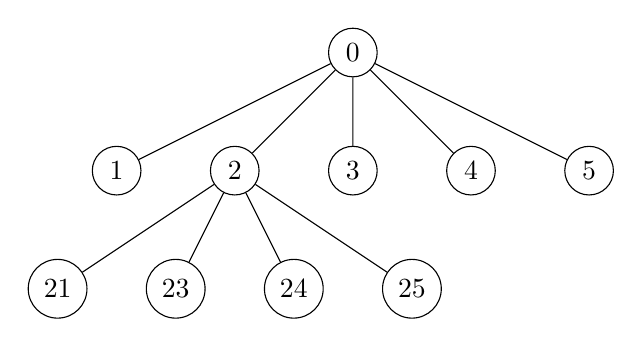
\begin{tikzpicture}[every node/.style={draw,circle}]
  \node (0) {0}
  child {node(1) {1}}
  child {node(2) {2}
    child {node(21) {21}}
    child {node(23) {23}}
    child {node(24) {24}}
    child {node(25) {25}}
  }
  child {node(3) {3}}
  child {node(4) {4}}
  child {node(5) {5}};
\end{tikzpicture}

The number of keys each node needs to keep will be increased
exponentially as $n - k$ becomes big. Up to $(7,10)$ threshold seems
practical.

\subsubsection*{DSA, ECDSA}
BFTKV implements a DSS threshold scheme introduced by Gennaro et
al.\ \cite{Gennaro}.
Since the scheme has a restriction such that $n \geq 2t$ in the $(t,
n)$-threshold scheme, we no longer be able to use the quorum threshold
for $(t, n)$. But, we follow the protocols between the client and a
quorum, i.e., the client sends a signing request to a quorum
(multicast the message to all quorum members), then collect the
responses. Our signing protocol consists of three phases:
\begin{enumerate}
\item Collect joint shared secrets generated by each quorum member
\item Distribute the secrets to the quorum and calculate
  $r=g^{k^{-1}} \bmod p \bmod q$ where $k$ is the
  joint Shamir's shared secret (i.e., $k = \sum k_i$)
\item Distribute r to the quorum and calculate $s=k(m+xr) \bmod q$
  from each $s_i=k_i(m+x_ir) \bmod q$ returned from each quorum member
\end{enumerate}
